\documentclass{article}
\usepackage[a4paper,left=3cm,right=3cm,top=1.5cm,bottom=2cm]{geometry}
\usepackage{amsmath}
\usepackage{amssymb}
\usepackage{hyperref}
\usepackage[english]{babel}

\usepackage{tikz-cd}
\usepackage{array}
\usepackage{graphicx}
\usepackage{mathtools}
\newcommand\mapsfrom{\mathrel{\reflectbox{\ensuremath{\mapsto}}}}
\setlength{\parindent}{0mm}
\usepackage{stmaryrd}

\usepackage{fontspec}
\setmainfont{Linux Libertine O}
\usepackage{unicode-math}
\setmathfont{Cambria Math}

\usepackage[nottoc]{tocbibind}

\begin{document}
\title{
\vspace{-1cm}
\textit{\small{Georgii Potoshin, 2025}}\\
\vspace{0.3ex}
\textit{\huge{Geometries and measures}}\vspace{1ex}
}
\date{\vspace{-5ex}}
\maketitle

\section{Introduction}
Geometric Measure Theory is indeed a geometric theory, because it is
driven by geometric ideas. A primary interest of this domain is to study how
measures can be used to investigate geometric properties of objects. With measures,
we can describe such things as shape convergence and local geometric properties
of objects and do not have any restrictions on smoothness.

\section{Conventions, acknowledged results and definition from analysis and measure theory}
\textbf{Convention:} To any product we associate morphisms denoted by $\pi_i$,
where $i$ is an index of product component we are projecting to or is the component
itself. For example for $A\times B$ we have $\pi_A:A\times B\rightarrow A$, for
$A^n$ we have $\pi_i:A^n\rightarrow A$ with $i\in\llbracket1,n\rrbracket$, for $\prod_{i\in I} A_i$
we have $\pi_{i_0}:\prod_{i\in I} A_i\rightarrow A_{i_0}$ for $i_0\in I$.
Similarly we introduce a notion $i$ for morphisms associated to coproducts.
Notions of morphisms $\pi$ and $i$ are reserved only for those needs.

\subsection{Measure theory}
\textbf{Definition:} \textit{An \textbf{outer measure} on $X$ is a set function on $X$ with
values in $[0,\infty]$ with
\begin{itemize}
    \item $\mu(\varnothing)=0$
    \item $E\subseteq\bigcup_{h\in\mathbb{N}}E_h\quad\Rightarrow\quad\mu(E)\leq\sum_{h\in\mathbb{N}}\mu(E_h)$
\end{itemize}
}

\vspace{2ex}
\textbf{Carathéodory's theorem:} \textit{If $\mu$ is an outer measure on $X$ and $\mathcal
M(\mu)$ is the family of those $E\subseteq X$ such that
\[\mu(F)=\mu(E\cap F)+\mu(F\setminus E),\quad\quad\forall F\subseteq X\]
then $\mathcal M(\mu)$ is a $\sigma$-algebra and $\mu$ is a measure on $\mathcal
M(\mu)$.}

\vspace{2ex}
\textbf{Definition:} \textit{$\mu$ is a \textbf{Borel measure} on a topological space $X$
if it is an outer measure on $X$ such that $\mathcal B(X)\subseteq\mathcal M(\mu)$.}

\vspace{2ex}
\textbf{Definition:} \textit{A measure $\mu$ is said to be \textbf{absolutely continuous
with respect to} measure $\lambda$ if for any set $A$, $\lambda(A)=0$
implies $\mu(A)=0$ and we write it $\mu << \lambda$.}

\vspace{2ex}
\textbf{Definition:} \textit{We say that a Borel measure $\mu$ is \textbf{regular} if
for every $F\subseteq X$ there exists a Borel set $E\in\mathcal B(X)$ such that
\[F\subseteq E,\quad\quad\quad\quad\quad\quad\mu(F)=\mu(E)\]}

\vspace{2ex}
\textbf{Definition:} \textit{An outer measure $\mu$ on $X$ is \textbf{locally finite} if
$\mu(K)<\infty$ for every compact set $K\subseteq X$.}

\vspace{2ex}
\textbf{Definition:} \textit{An outer measure $\mu$ is a \textbf{Radon measure} on a
topological space if it is locally finite, Borel regular measure on $X$.}

\vspace{2ex}
\textbf{Property of Radon measures on $\mathbb{R}^n$:} \textit{If $\mu$ is a Radon
measure on $\mathbb{R}^n$, then
\[
    \mu(E)=\inf\{\mu(A)\,|\,E\subseteq A,\,A\textnormal{ is open}\}
          =\sup\{\mu(K)\,|\,K\subseteq E,\,K\textnormal{ is compact}\}
\]}

\vspace{2ex}
\textbf{Definition:} \textit{A Borel measure $\mu$ on a metric space $X$ is
said to be a \textbf{doubling measure} if there exists a constant $C$ such that
\[0<\mu(B(x,2r))\leq C\mu(B(x,r))<\infty\]}

\subsection{Analysis}
\textbf{Definition:} \textit{For a function $f:X\rightarrow Y$ between metric spaces we can
define its \textbf{Lipschitz constant} $\text{Lip}(f) = \textnormal{inf}\{L\in
\mathbb{R}\,|\,d(f(x),f(y))\leq Ld(x,y) \forall x,y\in X\}$}

\vspace{2ex}
Geometric measure theory is based on few deep and not trivial results on space
$\mathbb{R}^n$ which I found in the book "Measure theory and fine properties
of functions". I took those results from that book with little modifications.

\vspace{2ex}
For a ball $B=B(x, r)$ of center $x$ and radius $r$ we shall note $\prescript{\epsilon}{}B
=B(x, (1+\epsilon)r)$ for every $\epsilon>0$. I chose the prefix notation to
avoid confusion with set power and Minkowski product.

\vspace{1ex}
\textbf{Vitali's covering lemma:} \textit{
Let $\mathcal{F}$ be any collection of nondegenearted closed balls in a metric
space $X$ with
\[ \sup\{\text{diam}\,B\,|\, B\in\mathcal{F}\}<\infty \]
Then for every $\epsilon>1$ there exist a countable family $\mathcal{G}$ of
disjoint balls in $\mathcal{F}$ such that
\[\bigcup_{B\in\mathcal{F}}B\subseteq\bigcup_{B\in\mathcal{G}}\prescript{2\epsilon}{}B\]}

\vspace{1ex}
\textbf{Proof:}
Set $D=\sup\{\text{diam}\,B\,|\,B\in \mathcal{F}\}$. Set
\[\mathcal{F}_j=\left\{B\in\mathcal{F}\,|\,\frac{D}{\epsilon^j}<\text{diam}\,B\leq\frac{D}{\epsilon^{j-1}}\right\},\quad j=1,2,\ldots\]
We define $\mathcal{G}_j\subseteq\mathcal{F}_j$ as follows
\begin{itemize}
    \item Let $\mathcal{G}_1$ be any maximal disjoint collection of balls in
        $\mathcal{F}_1$.

    \item Assuming $\mathcal{G}_1,\ldots,\mathcal{G}_{k-1}$ have been selected,
        we chose $\mathcal{G}_k$ to be any maximal disjoint subcollection of
        \[ \{B\in\mathcal{F}_k\,|\,B\cap B'=\varnothing\text{ for all }B'\in\bigcup_{j=1}^{k-1}\mathcal{G}_j\}\]
\end{itemize}
They exist by Zorn's Lemma. Finally, define $\mathcal{G}=\bigcup_{j\in\mathbb{N}^*}\mathcal{G}_j$
a collection of disjoint balls and $\mathcal{G}\subseteq\mathcal{F}$.

\vspace{1ex}
Proving that for each ball $B\in\mathcal{F}$, there exists a ball $B'\in\mathcal{G}$
such that $B\cap B'\neq\varnothing$ and $B\subseteq\prescript{\epsilon}{}B'$. Fix
$B\in\mathcal{F}$, there exists and index $j$ such that $B\in\mathcal{F}_j$ and
by maximality of $\mathcal{G}_k$ there exists a ball $B'\in\bigcup_{k=1}^j
\mathcal{G}_k$ with $B\cap B'\neq\varnothing$. But $\text{diam}\,B'>\frac{D}{\epsilon^j}$
and $\text{diam}\,B\leq\frac{D}{\epsilon^{j-1}}$; so that
\[ \text{diam}\,B\leq \frac{D}{\epsilon^{j-1}} < \epsilon\text{diam}\,B'\]
Thus $B\subseteq\prescript{2\epsilon}{}B'$.
\begin{center}
    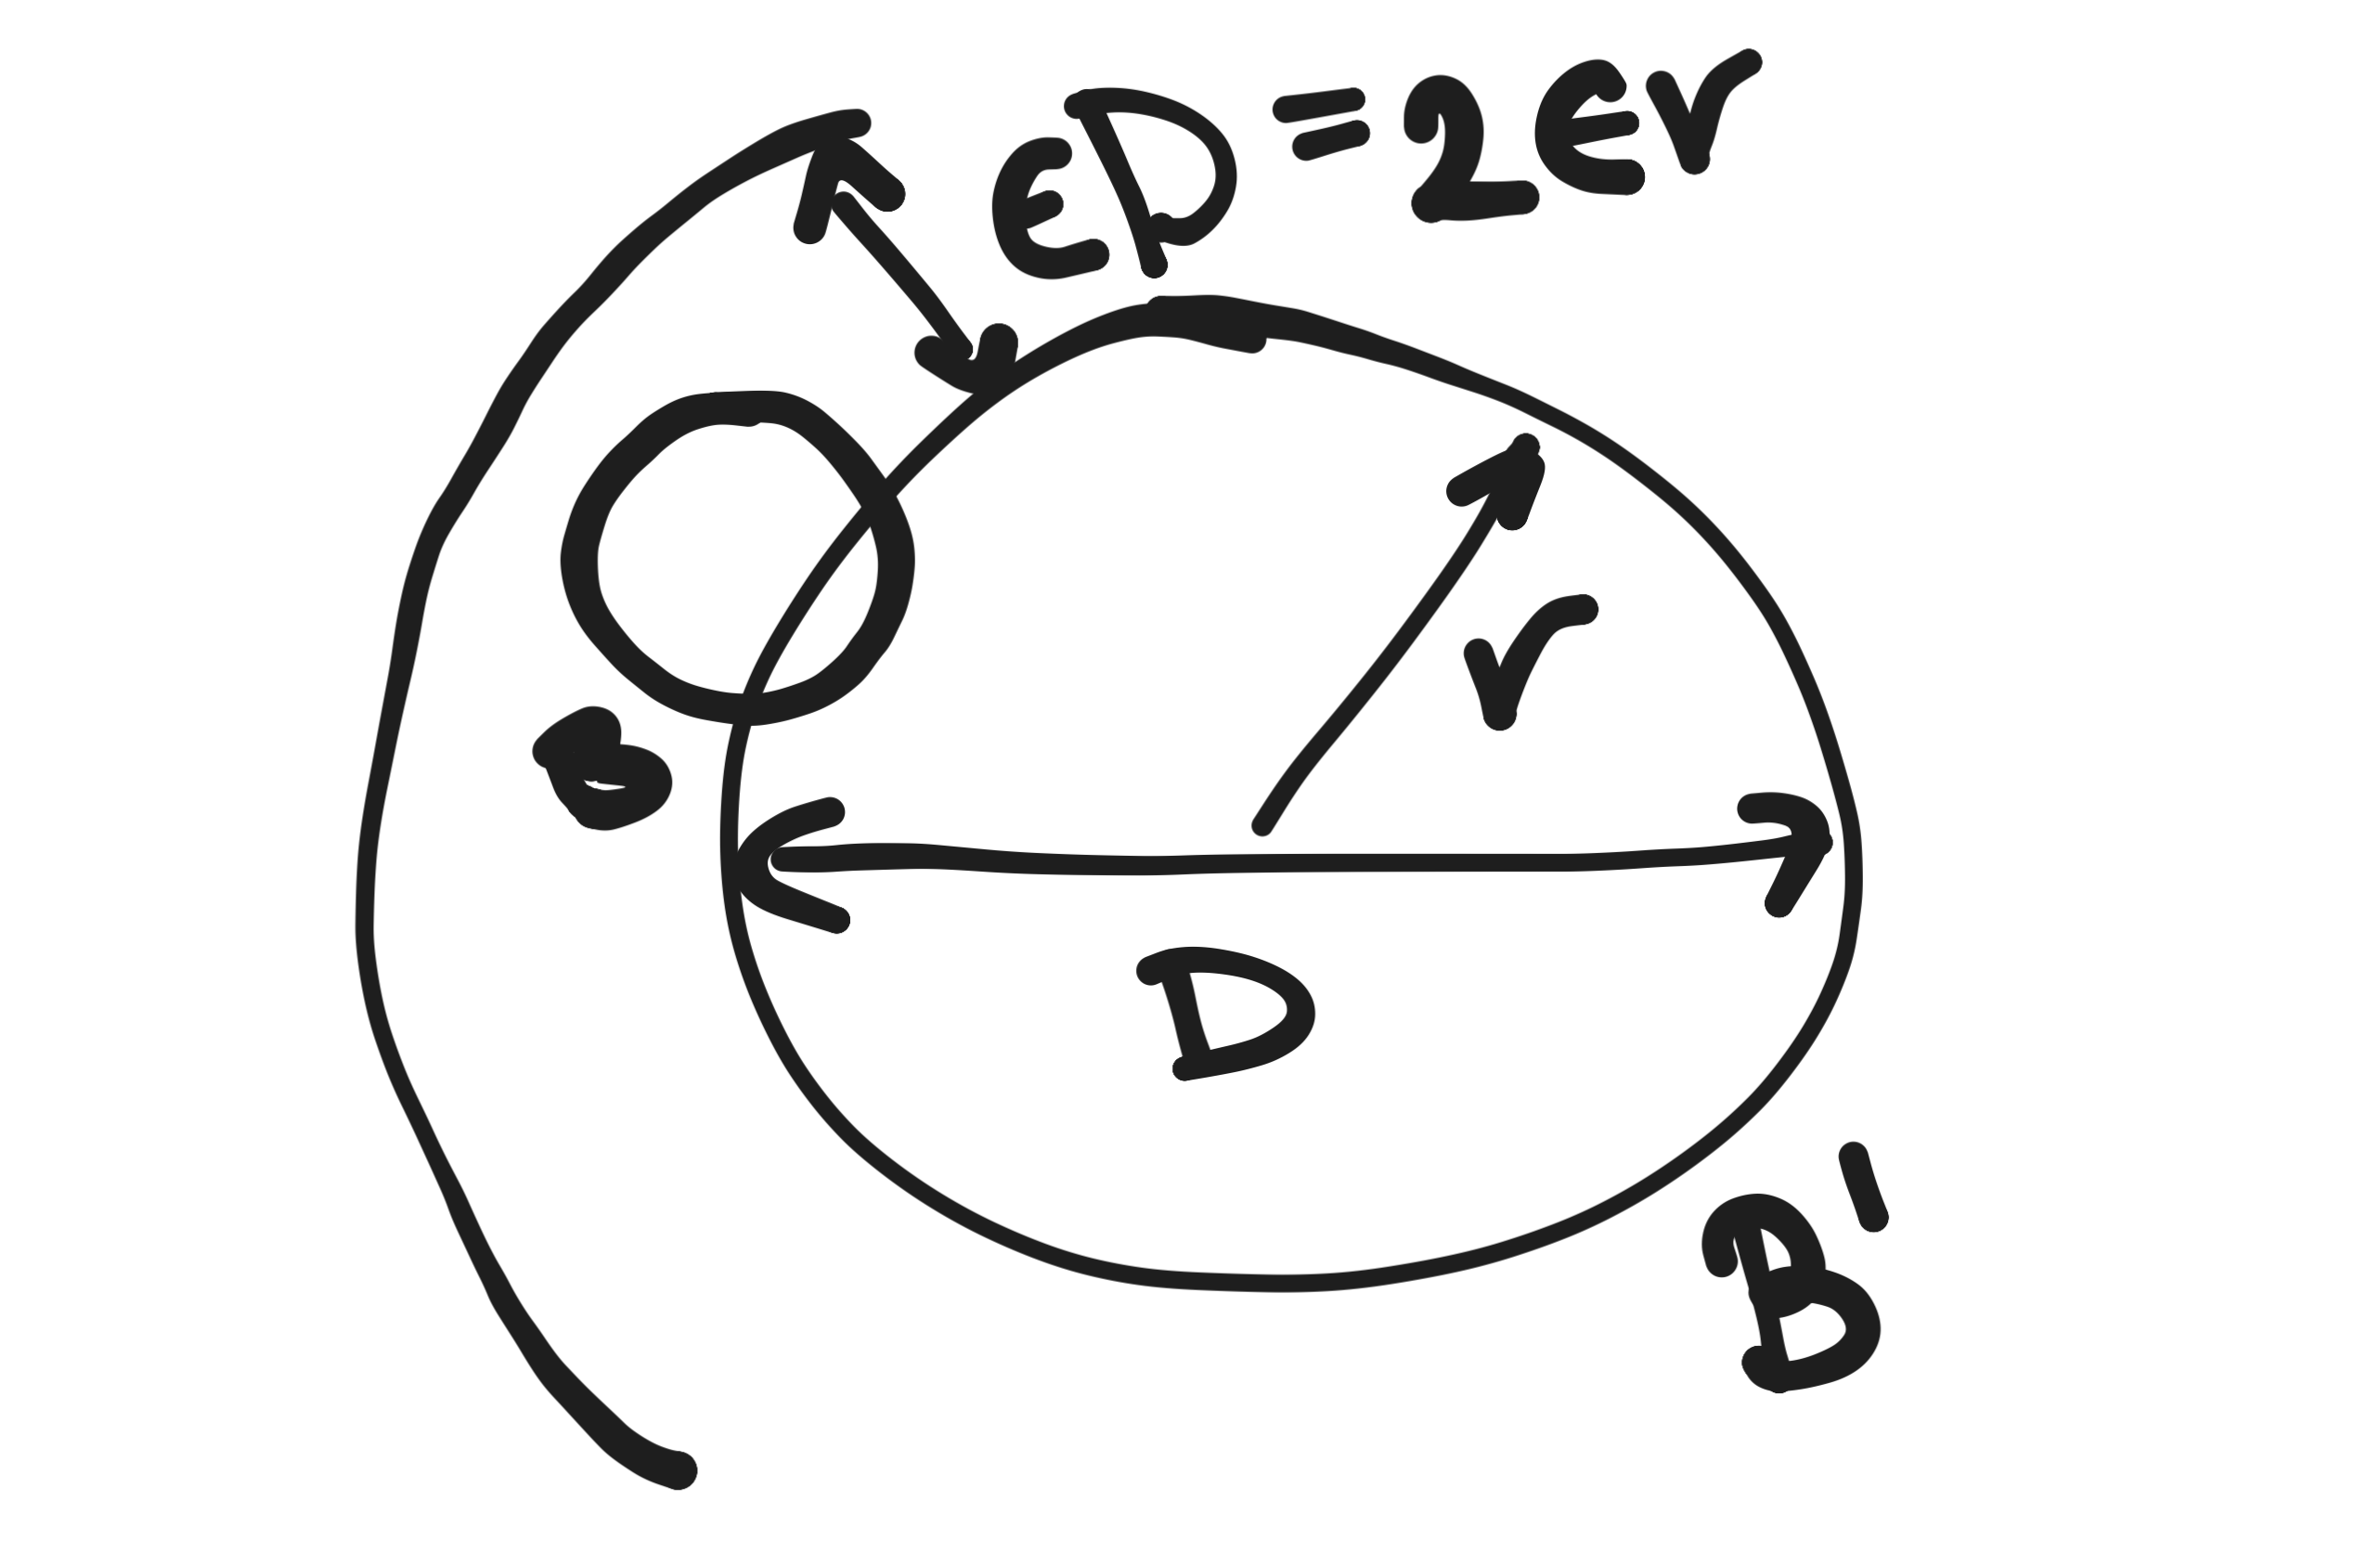
\includegraphics[scale=0.1]{Vitali.png}
\end{center}
\vspace{1ex}
\textbf{Remark:} This is a generalised version of the proof from the book
"Measure theory and fine properties of functions" where it is done for the
smallest integral case $\epsilon = 2$. The generalised proof shows the reason
why the final dilatation is $5 = 1+2\epsilon$, but actually it is true for
dilatation $>3$ and the smallest such integer is 4. An interesting question is
whether there is continuity and can we take a limit and get this result also
for 3.

\vspace{2ex}
\textbf{Besicovitch’s Covering Theorem:} \textit{There exists a constant $N_n$, depending
only on the dimension $n$ with the following property:}

\vspace{1ex} \textit{
If $\mathcal{F}$ is any collection of non-degenerated closed balls in
$\mathbb{R}^n$ with
\[\sup\{\textnormal{diam}\,B\,|\,B\in\mathcal F\}<\infty\]
and $A$ is the set of centers of balls in $\mathcal F$, then there $N_n$
countable collections $\mathcal{G}_1,\ldots,\mathcal{G}_{N_n}$ of disjoint
balls in $\mathcal{F}$ such that
\[A\subseteq\bigcup_{i=1}^{N_n}\bigcup_{B\in\mathcal{G_i}}B\]}

\vspace{1ex}
\textbf{Proof:} take a look at \cite{evans_gariepy}.

\vspace{2ex}
\textbf{Definition:} \textit{A cover of $A$ by a family $B$ is called \textbf{fine}
if for any $x\in A$ we can find a covering set from $B$ of arbitrary small
diameter.}

\vspace{2ex}
\textbf{Filling open sets with balls theorem:} \textit{Let $\mu$ be a Borel measure on
$\mathbb{R}^n$, and $\mathcal{F}$ any collection of non-degenerated closed balls.
Let $A$ denote the set of centers of the balls in $\mathcal F$. Assume
\[\mu(A)<\infty\]
and $\mathcal F$ is a fine cover of $A$. Then for each open set $U\subseteq\mathbb{R}^n$, there
exists a countable collection $\mathcal G$ of disjoint balls in $\mathcal F$ such that
\[\bigcup_{B\in\mathcal G} B\subseteq U\]
and
\[\mu\left((A\cap U)\setminus\bigcup_{B\in\mathcal G}B\right)=0.\]}

\vspace{1ex}
\textbf{Proof:}

\vspace{2ex}
\textbf{Whitney's extension theorem:}\textit{
Let $C\subseteq \mathbb{R}^n$ be a closed set and $f:C\rightarrow\mathbb R$,
$d:C\rightarrow\mathbb{R}^{n*}$ be continuous functions. We shall use notions}
\begin{align*}
    &R(y,x)=\frac{f(y)-f(x)-d(x)(y-x)}{|x-y|},\quad\forall x,y\in C, x\neq y \\
    &\rho_k(\delta)=\sup\{|R(x,y)|\, |\, 0<|x-y|\leq\delta, x, y\in K\}
\end{align*}
\textit{if we suppose that for every compact $K\subseteq C$}
\begin{equation}
\rho_K(\delta)\rightarrow 0\text{ as }\delta\rightarrow 0
\end{equation}

\textit{Then there exists a fuction $\overline f\in\mathcal{C}^1(\mathbb{R}^n,\mathbb{R})$
and $D\overline f|_C=d$.}

\vspace{1ex}
\textbf{Remark:}
I seek to give a more explicit version of the proof given in the book "Measure
theory and fine properties of functions". In books that looked at about
geometric measure theory this proof usually is not stated and pointed to the
book of Federer wheres at least in version of that book the theorem is proved
in much more general context and the theorem statement differs from the one we
want.

\vspace{1ex}
\textbf{Proof:} You can find one in this book \cite{evans_gariepy}, it's quite
complecated and I do not fill empowered to invate on it and it is not a purpose
of this paper.


\vspace{2ex}
\textbf{Lipschitz function extension theorem:} \textit{Let $X$ be a metric space,
$A\subseteq X$ and $f:A\rightarrow\mathbb{R}$. Then there exists a Lipschitz
function $\overline f:X\mapsto\mathbb{R}$ such that $\textnormal{Lip}(f)=\textnormal{Lip}
(\overline f)$ and $\overline f|_A=f$.}

\vspace{1ex}
This is a proof from "Simons Lectures on geometric measure theory". Let's set
$L=\text{Lip}(f)$. Then we define
\[\overline f(x) = \text{inf}_{y\in A}(f(y)+Ld(x,y)\]
By the definition, for all $x\in A$, $\overline f(x)\leq f(x)$ as in particular
we can chose $y=x$.
Furthermore, for all $a,b\in A$ and $x\in X$, we have an inequality for a
Lipschitz function $f(b)-f(a)\leq Ld(b,a)\leq Ld(b,x)+Ld(a,x)$ and thus we have
\[ f(a)+Ld(a,x)\geq f(b)-Ld(b,x)\] 
and if we apply an infinum over a, we have $\overline f(x)\geq f(b)-L(b,x)$ and
if $x\in A$ we can chose $b=x$ and we have an inequality in the other direction
and thus the equality $\overline f(x)=f(x)$.

\vspace{1ex}
Now we check the Lipschitz constant
%\begin{align*}
%
%\end{align*}

\vspace{1ex}
\textbf{Consequence:} \textit{Let $X$ be a metric space, $A\subseteq X$ and
$f:A\rightarrow\mathbb{R}^n$. Then there exists a Lipschitz
function $\overline f:X\mapsto\mathbb{R^n}$ such that $\overline f|_A=f$}

\vspace{1ex}
Let's set $\overline f = (\overline f_i)_i$ extension by coordinate functions. 

\vspace{1ex}
\textbf{Remark:} I was thinking about extending the theorem to the case where
function take vector values, but I can only prove it for the maximum norm.

\subsection{Differentiation of Radon measure and Radon-Nikodym Theorem}
\textbf{Remark:} That section is an adopted version of paragraph 1.6 from the
book "Measure theory and fine properties of functions" for vector measures.

\vspace{2ex}
\textbf{Definition:} \textit{Let $\mu$ and $\nu$ be Radon measures on $\mathbb{R}^n$.
Then we can define upper and lower derivatives of $\nu$ by $\mu$ by
\begin{align*}
    &\overline D_\mu\nu(x) =
    \left\{\begin{array}{rcl}
        \limsup_{r\rightarrow0}\frac{\nu(B(x,r))}{\mu(B(x,r))} & \textnormal{if }\mu(B(x,r))>0\textnormal{ for all }r>0\\
        +\infty & \quad\textnormal{if }\mu(B(x,r))=0\textnormal{ for some }r>0
    \end{array}\right.\\
    &\underline D_\mu\nu(x) =
    \left\{\begin{array}{rcl}
        \liminf_{r\rightarrow0}\frac{\nu(B(x,r))}{\mu(B(x,r))} & \textnormal{if }\mu(B(x,r))>0\textnormal{ for all }r>0\\
        +\infty & \quad\textnormal{if }\mu(B(x,r))=0\textnormal{ for some }r>0
    \end{array}\right.
\end{align*}
If $\overline D_\mu\nu(x)=\underline D_\mu\nu(x)<+\infty$ then we say that $\nu$
is \emph{differentiable} with respect to $\mu$ at x and we write
\[D_\mu\nu(x)=\overline D_\mu\nu(x)=\underline D_\mu\nu(x)\]
}

\vspace{1ex}
\textbf{Definition:} \textit{Let $\mu$ be Radon measure and $\nu$ be a vector measure on
$\mathbb{R}^n$. Then we define a derivatives as
\[
    D_\mu\nu(x) =
    \left\{\begin{array}{rcl}
        \lim_{r\rightarrow0}\frac{\nu(B(x,r))}{\mu(B(x,r))} & \textnormal{if }\mu(B(x,r))>0\textnormal{ for all }r>0\\
        +\infty & \quad\textnormal{if }\mu(B(x,r))=0\textnormal{ for some }r>0
    \end{array}\right.
\]
}

\vspace{1ex}
\textbf{Upper and lower derivatives lemmas:} \textit{For Radon measures and
$\alpha\in\mathbb{R}_{>0}$ we have
\begin{itemize}
    \item $A\subseteq\{x\in\mathbb{R}^n\,|\,\underline D_\mu\nu(x)\leq\alpha\}$ implies $\nu(A)\leq\alpha\mu(A)$.
    \item $A\subseteq\{x\in\mathbb{R}^n\,|\,\overline D_\mu\nu(x)\geq\alpha\}$ implies $\nu(A)\geq\alpha\mu(A)$.
\end{itemize}
}

\vspace{1ex}
\textbf{Proof:}
We may assume that measures are finite, otherwise we can always take
restriction to compact sets. For $\epsilon>0$ and open $U\supseteq A$, where
$A$ satisfies the first hypothesis. We set
\[\mathcal{F}=\{B\;|\;B=B(a, r), a\in A, B\subseteq U, \nu(B)\leq(\alpha+\epsilon)\mu(B)\}\]
This family has the following properties. We have infinitely many balls in it
around each point with diminishing radius, because we have lower limit $\leq a$
there. Then $\inf\{r\;|\;B(a,r)\in\mathcal F\}=0$ for each $a\in A$ and hence
\emph{Filling Theorem} provides us with a countable collection $\mathcal G$ of
disjoint balls in $\mathcal F$ such that
\[\nu\left(A-\bigcup_{B\in\mathcal G}B\right)=0\]
Then
\[\nu(A)\leq\sum_{B\in\mathcal G}\nu(B)\leq(\alpha+\epsilon)\sum_{B\in G}\mu(B)
\leq(\alpha+\epsilon)\mu(U)\]
This esteem is valid for each open set $U$ and thus as we have a radon measure,
we have $\nu(A)\leq(a+\epsilon)\mu(A)$, which proves the first bullet.

\vspace{1ex}
To prove the second bullet we do a similar routine. We pose similar $U$ and
$\epsilon$. We slightly change $\mathcal F$
\[\mathcal{F}=\{B\;|\;B=B(a, r), a\in A, B\subseteq U, \nu(B)\geq(\alpha-\epsilon)\mu(B)\}\]
and we find $\mathcal G$ for $\mu$ instead of $\nu$ such that
\[\mu\left(A-\bigcup_{B\in\mathcal G}B\right)=0\]
Then
\[\mu(A)\leq\sum_{B\in\mathcal G}\mu(B)\leq1/(\alpha-\epsilon)\sum_{B\in G}\nu(B)
\leq1/(\alpha-\epsilon)\nu(U)\]
and we get the second bullet.

\vspace{2ex}
\textbf{Differentiating measures theorem:} \textit{Let $\mu$ and $\nu$ be Radon
measures on $\mathbb{R}^n$. Then
\begin{itemize}
    \item $D_\mu\nu$ exists and is finite $\mu$-a.e.
    \item $D_\mu\nu$ is $\mu$-measurable
\end{itemize}
}

\vspace{2ex}
\textbf{Remark:} This is a brilliant version with a proof of Radon Nikodym
Theorem by von Neumann, that will suffice our need for representing vector measures.

\vspace{1ex}
\textbf{Radon-Nikodym Theorem:} \textit{Let $\mu$ and $\nu$ be finite measures
on $(\Omega, \mathcal F)$ then there exists a non-negative measurable function
$f$ and a $\mu$-null set $B$ such that
\[\nu(A) = \int_Af\,d\mu+\nu(A\cap B)\]
for each $A \in \mathcal F$.
}

\vspace{1ex}
\textbf{Proof:} Let $\pi=\mu+\nu$ and consider $T(f)=\int fd\nu$. Then for
every $f\in L^2(\pi)$ we have $f\in L^1(\nu)$ and since measures are finite
$f\in L^1(\pi)$ and thus in $L^1(\nu)$, then
\[|T(f)|=|\int f\,d\nu|\leq\|f\|_{L^2(\nu)}\|1\|_{L^2(\nu)}\leq C\|f\|_{L^2(\pi)}\]
where $C$ is a constant. Thus $T$ is a continuous operator on $L^2(\pi)$ and by
Reisz representation theorem for Hilbert spaces we find a function $h\in L^2(\pi)$
such that
\[T(f)=\int f\,d\nu=\int fh\,d\pi\]
Now consider the following sets
\[N=\{h<0\},\quad M=\{0\leq h<1\},\quad B=\{h\geq 1\}\]
Then
\[0\geq\int_N h\,d\pi=\int\chi_N h\,d\pi=\nu(N)\geq 0\]
Thus we have $\nu(N)=0$ and since $h<0$ on $N$ and $\int h\,d\mu=0$ we have
$\mu(N)=0$ also.

\vspace{1ex}
Now let's study $B$. We have
\[\nu(B)=T(\chi_B)=\int_Bh\,d\mu+\int_B h\,d\nu\geq\nu(B)+\mu(B)\]
thus $\mu(B)=0$.

For the last let we set $M_n=\{0\leq h\leq1-1/n\}$ and from representation of
$T$ with $h$ we have $\int(1-h)f\,d\nu=\int hf\,d\mu$ and why apply it to
\[\nu(M_n)=\int\frac{\chi_{M_n}}{1-h}(1-h)\,d\nu=\int h\frac{\chi_{M_n}}{1-h}\,d\mu\]

Let $f=\frac{h}{1-h}$ then by applying monotone convergence and recalling that
$\mu(B)=\mu(N)=0$ we have
\[\nu(M\cap A)=\int_A f\,d\mu\]

Finally for all $A\in\mathcal F$ we have
\[\nu(A)=\nu(A\cap N)+\nu(A\cap M)+\nu(A\cap B) = \int_A f\,d\mu+\nu(A\cap B)\]

\vspace{2ex}
\textbf{Corollary:} If $\mu >> \nu$, then $\nu(A)=\int_A f\,d\mu$

\vspace{1ex}
It's evident as $\mu(B)=0\Rightarrow\nu(B)=0$ then. 

\vspace{2ex}
\textbf{Remark:} If $\mu$ and $\nu$ are Radon measures, then $f=D_\mu\nu$.

\vspace{2ex}
\textbf{Corollary:}
This gives us a representation of a vector valued measure $\mu$ as $\mu=f\,|\mu|$.
And we can define the integration with respect to such measure as
\[
\int g\,d\mu = \int g\cdot f\,d|\mu|
\]

\vspace{2ex}
In the context of geometric measure theory we are interested in the vector
space $E=\mathcal{C}^0_c(X, \mathbb{R}^m)$ with the supremum norm.
Then its dual space is $E^*=\{L:E\rightarrow\mathbb{R}\,|\,L\text{ is linear
and continious}\}$ is a vector space of bound linear functionals. Then on the $E^*$ from 
now and on we will consider the weak-$*$ topology.



\section{Hausdorff measure}
The Hausdorff measure generalizes the notion of measure for lower-dimensional
objects in a higher-dimensional space or even in an arbitrary metric space.
The idea is essentially similar to the construction of Lebesgue measure, and
the general case is called the Carathéodory construction. The difference is
that we measure sets by their diameter, attributing to each an s-dimensional
"volume" based on its diameter raised to the power of s. For this construction,
we define a cover of E by sets of diameter less than δ as a δ-cover of E. And
we consider only countable covers. We note that
\[\mathcal{H}_\delta^s(E)=\inf_{C}\sum_{I\in C}\omega_s\left(\frac{\text{diam}(I)}{2}\right)^s\]
where $s\in\mathbb{R}_{\geq 0}$ is a dimension, $\omega_s\in\mathbb{R}$ is a
coefficient, preferably continuous or smooth as a function of $s$, and $C$ is a
$\delta$-cover of $E$. We may assume that
\[\omega_s = \frac{\pi^{s/2}}{\Gamma(1+s/2)}\]
We define the Hausdorff measure as a limit of the previous value. It exists
because $\mathcal{H}_\delta^s(E)$ is an increasing function of $\delta$. We note
\[\mathcal{H}^s(E)=\lim_{\delta\rightarrow0^+}\mathcal{H}^s_\delta(E)\]

I shall introduce the notion of $s$-variation of a cover $S$ as
\[\text{Var}^s(S)=\sum_{I\in S}\omega_s\left(\frac{\text{diam}(I)}{2}\right)^s\]

\textbf{Proposition:} \textbf{For a natural $n\geq 0$, $\omega_n$ is a volume of a unit
$n$-dimensional ball.}
\vspace{1ex}

\subsection{Properties of Hausdorff measure}

\textbf{Proposition:} \textit{Hausdorff measure is a Borel measure.}

\vspace{2ex}
\textbf{Proposition:} $\mathcal H^0$ is the counting measure.

\vspace{2ex}
\textbf{Proposition:} \textit{In the definition of Hausdorff measure we can consider
only closed or open sets.}

\vspace{2ex}
\textbf{Proposition:} \textit{Hausdorff measure of dimension $m\in N$ coincide on
$m$-dimensional affine subspaces with their Lebesgue measure.}

\vspace{2ex}
\textbf{Proposition:} \textit{The $n$-dimetional Hausdorff measure traced to a
$n$-dimentional $\mathcal{C}^1$-submanifold of $R^m$ induces the area measure
on this submanifold and coincides with the integral measure via parametrisation
on it.}

\vspace{2ex}
\textbf{Proposition:} \textit{A restriction of $\mathcal H^s$ on a locally
$\mathcal H^s$-finite set is a Radon measure.}

\vspace{1ex}
\textbf{Remark:} Proofs to those proposition can be found in the book "Geometric
measure theory" be Francesco Maggi \cite{maggi}.

\vspace{2ex}
\textbf{Definition:} \textit{Let $E$ be a Borel subset of a metric space $X$.
The \textbf{upper $d$-dimensional density} (with respect to $\mathcal H^d$) of $E$ at
the point $x$ is defined by setting
\[\Theta^*_d(E,x)=\limsup_{r\rightarrow 0}\frac{\mathcal H^d(E\cap B_c(x,r))}{\omega_dr^d}\]}

\vspace{2ex}
\textbf{Theorem:} \textit{Let $E$ be a Borel subset of a metric space $X$, and
assume that $E$ is locally $\mathcal H^d$-finite. Then the following properties
hold true:
\begin{enumerate}
    \item The upper density of external points is almost everywhere zero,
        $\Theta^*_d(E, x)=0$ for $\mathcal H^d$-almost every $x\in E^c$.
    \item The upper density is bounded from below, $\frac{1}{2^d}\leq\Theta^*
        _d(E,x)$ for $\mathcal H^d$-almost every $x\in E^c$.
    \item If $X\cong\mathbb R^n$, then the upper density is bounded from above
        by 1, $\Theta^*_d(E,x)\leq 1$ for $\mathcal H^d$-almost every $x\in E$.
    \item If $X$ is a generic metric space, then the upper density is bounded
        from above by a slightly different constant, $\Theta^*_d(E,x)\leq3^d$
        for $\mathcal H^d$-almost every $x\in E$.
\end{enumerate}
}

\vspace{1ex}
\textbf{Proof:} Proofs of propositions 2-3 can be found in \cite{giovanni_alberti}
on page 48.

\vspace{1ex}
\begin{enumerate}
    \item The core of this proof is to use regularity of $\mu:=\mathcal H^d\,
        \llcorner E$ and Vitali's lemma. Let $E_t:=\{x\in E^c\,|\,\Theta^*_d(E,x)>t\}$
        and we prove that it's $\mathcal H^d$-null for $t>0$. From the
        definition of $E_t$ we know that $E$ is highly concentrated around of
        points of $E_t$. Thus in some sense we can replace a study of $E_t$ with
        study of covers. Let $A\supseteq E_t$ be an open neighborhood of $E_t$.
        Then we take $\mathcal F:=\{\overline{B(x,r)}\subset A\,|\,x\in E_m\;\&
        \;\mathcal H^d(\overline{B(x,r)}\cap E)>t\omega_dr^d\}$. In this family
        we can leave only balls of diameter $<1$. Then for \textbf{Vitali's
        Covering Lemma} we can choose a dilation coefficient $k\in(3,+\infty)$
        and we fix ball dilatation procedure with coefficient $k$ by $B\mapsto
        \widehat B$. Lemma gives us a disjoint subfamily $\mathcal G$ such that
        after $\widehat\cdot$ it covers $E_t$. And we have a following
        inequality
        \begin{align*}
            \mu(A)\geq\sum_{B\in\mathcal G}\mu(B)\geq t\omega_d\sum_{B\in
            \mathcal G}r(B)^d=\frac{t}{k^d}\omega_d\sum_{B\in\mathcal G}r(
            \widehat B)^d\geq\frac{t}{k^d}\mathcal H^d_1(E_n)
        \end{align*}
        And as we can chose $\mu(A)$ arbitrary small, $\mathcal H^d_1(E_t)=0$ and thus
        $\mathcal H^d(E_t)=0$.
    \item No proofs for now
    \item No profs for now
    \item If we follow a similar construction as in the proof of the first
        proposition for a set $E_t:=\{x\in E\,|\,\Theta^*_d(E,x)>t\}$, then
        at the end we'll get
        \[\mathcal H^d(E_m)\geq\frac{t}{k^d}\mathcal H^d(E_m)\]
        and if $t>k^d$ we get $\mathcal H^d(E_m)=0$, and as it is true for all
        $k>3$, we have $\Theta^*_d(E,x)\leq3^d$. Remarque that usually there
        are no generalisation in Vitali's lemma and one usually proves for 5
        instead of 3.
\end{enumerate}

\subsection{Hausdorff dimension}
To a set $S$ we can associate a number $s=\text{inf}\{a\geq 0\,|\,\mathcal{H}^a
(S)=0\}$. It's called its Hausdorff dimension.

\vspace{2ex}
\textbf{Proposition:} \textit{If $E\subseteq\mathbb R$ then $\dim(E)\in [0, n]$.
Moreover $\mathcal H^s(E)=\infty$ for every $s<\dim(E)$ and $\mathcal H^S(E)\in
(0,\infty)$ implies $s=\dim(E)$.}

\vspace{2ex}
\textbf{Proposition:} \textit{If $A$ is an open set in $\mathbb R^n$, then $\dim
(A) = n$.}

\vspace{2ex}
\textbf{Proposition:} \textit{For a Lipschitz function $f:\mathbb{R}^n\rightarrow
\mathbb{R}^m$ we have the following inequality
\[ \mathcal{H}^s(f[E])\leq\text{Lip}(f)^s\mathcal{H}^s(E) \]
for every $s>0$ and $E\subseteq\mathbb{R}^n$ and $\text{dim}(E)<\text{dim}(f[E])$.}

\subsection{Dimension of cantor sets}
Here we compute the dimension of generalized set. Let $n\in\mathbb{N}$ and
$m\in\mathbb{N}^*$ so that $2m<n$. Then we can define $C_k$ ($k\in\mathbb{N}$)
define recursively by agreeing that $C_0=\{[0,1]\}$ and we obtain $C_{k+1}$ from $C_k$
by cutting out the open middle part from each segment of $C_k$ and living side parts
of length $m/n$ of original interval. We will note $C=\lim C_k=\bigcap C_k$.
\begin{center}
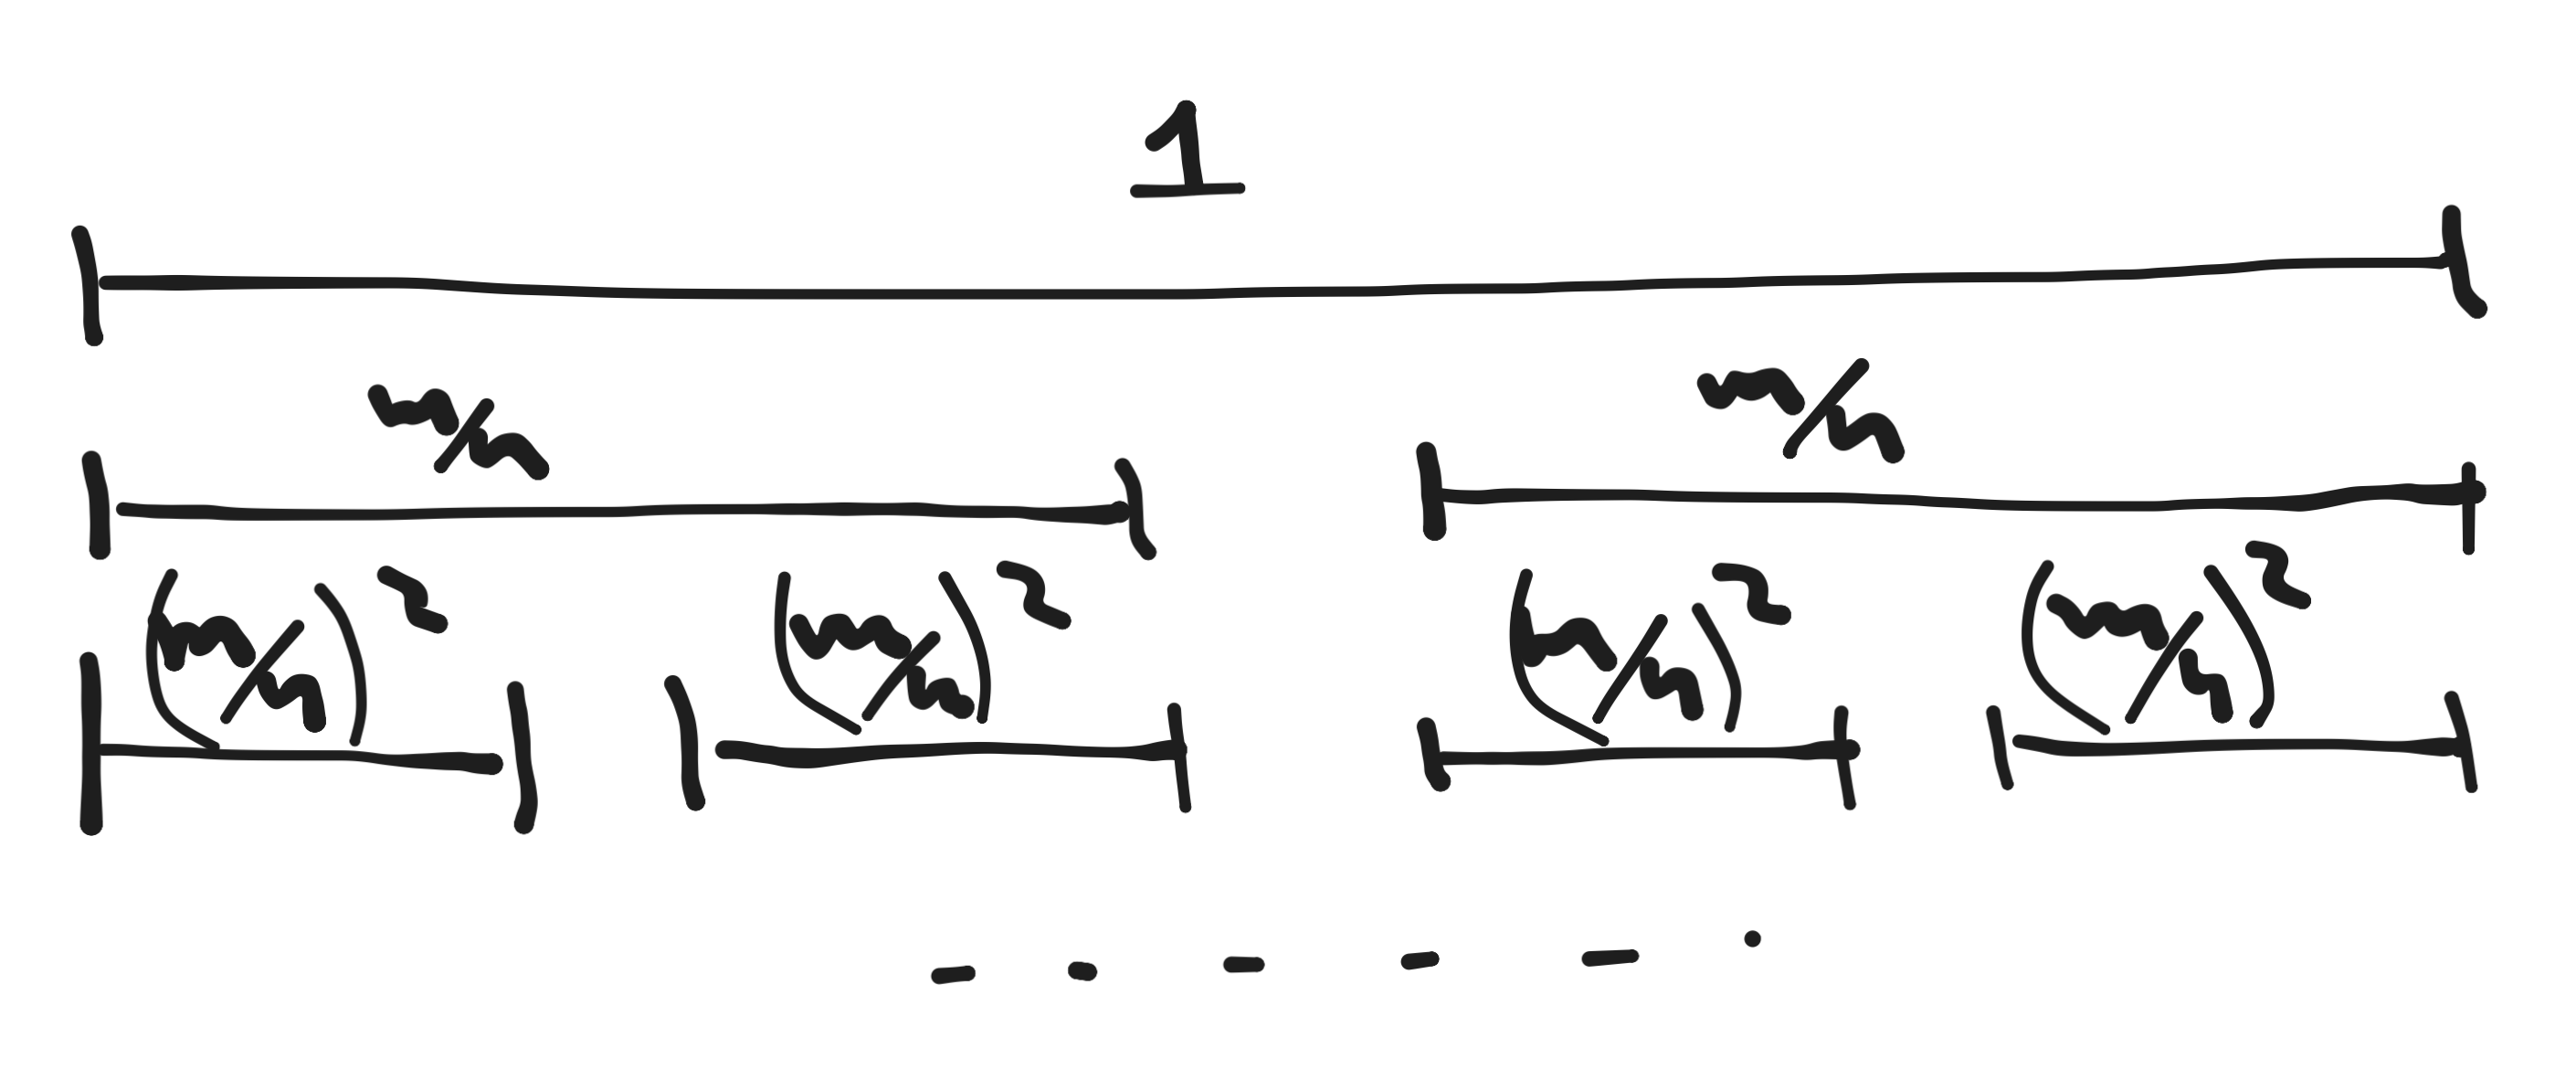
\includegraphics[scale=0.15]{cantor.png}
\end{center}
Obviously $C_k$ is a $(m/n)^k$-cover of $C$, so
\[ \mathcal{H}_{(m/n)^k}^s \leq \sum_{I\in C_k}\omega_s(\frac{\text{diam}(I)}{2})^s
=\omega_s2^k((m/n)^k)/2)^s=\omega_s/2^s(2(m/n)^s)^k \]
And if $s>\text{log}_{n/m}(2)$ we have right side approaching 0 as $k$ tends to
infinity. That means that $\text{dim}(C)\leq\text{log}_{n/m}(2)$.


Now we need to prove the inequality in the other direction. Let $s=\text{log}_
{n/m}(2)$. And let $S$ be a $(m/n)^k$-cover of $C$. In fact by the construction
$C$ is an intersection of compacts on a real line, so is compact. And by one of
the previous propositions we can conceder only open covers. Then by compactness 
we can leave only a finite number of sets in $S$ and this way we reduce its 
Hausdorff variance and we can extend the resting elements to closed intervals
of the same diameter. This does not change the variance. The new cover is noted
by $S'$. Now in every interval of $S'$ we can find 2 maximal intervals from some
$C_i$ and $C_j$, so the they are disjoint. If we can't do that, then there are no points
of $C$ in this interval and we can throw away that set also. So now we have 2 
maximal intervals $J$ and $J'$ in $I$. They are ordered. Between them we
have an interval $K$ and as they are maximal $I\setminus J\setminus K\setminus J'$ does not contain
any points from $C$ and we can through those parts away from the covering.
By the construction
\[|J|,|J'|\leq \frac{m}{n}\cdot \frac{n}{n-2m}|K|=\frac{m}{n-2m}|K|\]
Now we have $1/2(|J|+|J'|) \leq \frac{m}{n-2m}|K|$
\[|I|^s=(|J|+|J'|+|K|)^s\geq((1+\frac{n-2m}{2m}))(|J|+|J'|))^s=(\frac{n}{m}1/2(|J|+|J'|))^s=2(1/2(|J|+|J'|))^s\geq|J|^s+|J'|^s\]
Where the last step is done by concavity of function $x\mapsto x^s$.
That means that we can reduce this any cover to a $C_k$ cover which has a
smaller $s$-variation. That means that for dimension $s=\text{log}_{n/m}(2)$
the $\mathcal{H}^s(C)$ is finite as the $s$-variation of $C_k$ is always $
\omega_s/2^s$.

\vspace{1ex}
\textbf{Remark:} This is a variation on the proof given in the book "The geometry
of fractal sets" by K. J. Flaconer, generelised to the case of arbitrary $m$ and
$n$. In this book the proof is done for the case $m=1$, $n=3$.

\vspace{1ex}
\textbf{Proposition:} \textit{There is a subset of $[0,1]$ with а Hausdorff dimension
$1$, but Lebesgue measure 0.}

\vspace{1ex}
To show that we shall use Cantor's sets. Let $C_{m/n}$ be a set discussed in a
previous paragraph. Then $S=\bigcap C_{m/(2m+1)}$ is a set of dimension $1$. As
for every $0\leq s<1$ there is such $m$, that $\text{log}_{n/m}(2)=\text{log}_{
(2m+1)/m}(2)>s$, as $\text{log}_{(2m+1)/m}(2)\rightarrow 1$. And thus $\mathcal
{H}^s(S)>\mathcal{H}^s(C_{m/(2m+1)})=\infty$.


\section{Convergence of measures}
Measures not only allow us to compute integrals, but they can also be used to
model geometric figures and to test different properties of these figures. One
of the fundamental ideas at the heart of geometric measure theory is that one
can replace figures with the measures induced on these figures.
\[E\rightsquigarrow \mu\,\llcorner\hspace{-1mm}E\]
Now, we need to compare two figures. To do this, we can compare the values of
integrals of functions with respect to associated measures; in other words, we will
treat measures as linear functionals. Furthermore, if two figures are close to
one another, then we want their associated measures to yield sufficiently close
values. This implies that we want the function values to remain bounded in small
neighborhoods and not vary too much. Therefore, we only consider continuous
functions. Lastly, since we want to be able to work with possibly unbounded
figures, we would like the integration of measures with respect to functions to
be well-defined and finite. Thus, we only use continuous functions with compact
support, $\mathcal C_c(X)$.

\vspace{1ex}
This allows us to establish a notion of convergence of shapes, equivalent to a
convergence of measures. We'll see examples of this later, but for now, I'd
like to specify the type of convergence we'll be using.

We are treating measures as linear functionals on the space $\mathcal C_c(X)$.
In this context, convergence is defined by the behavior of these functionals on
each test function; specifically, we are considering that the integral values
converge for every function in $\mathcal C_c$. Such convergence is called 
weak-* convergence. Before discussing this convergence further, I shall first
demonstrate that there is a space of measures which serves as the dual space to
$\mathcal C_c$.

\subsection{Topologies on spaces $E$ and $E^*$}
For topological spaces $Y_i$ and a set of functions $f_i:X\rightarrow Y_i$, we can
define the smallest, coarsest topology on $X$ that makes these functions continuous.
By definition such topology is $\tau(\{f_i\})=\bigcap\{\tau\,|\,
\tau$ is a topology on $X$ and $f_i$ are continuous$\}$. As an
example, the product topology is exactly $\tau(\{\pi_i\})$, where $\pi_i$ are
canonical projections.
\vspace{1ex}

\textbf{Proposition:} \textit{Let $\tau$ be a topology on $X$. Then $\tau=\tau(\{f_i\})$
if and only if every function $g:W\rightarrow X$ such that $f_i\circ g$ are
continuous is continuous.}
\vspace{1ex}

\textbf{Remark:} This is a well-known property of caorsest topology, but I
checked that it is also an alternative characterisation of such topology.

If $\tau=\tau(\{f_i\})$ and $g:W\rightarrow X$ is such function that $f_i\circ
g$ are continuous. It's sufficient to check that for all elements of prebase
of $\tau(\{f_i\})$ the inverse image is open, but the prebase consists of
elements of the form $f_i^{-1}[U]$ and its inverse image is $(f_i\circ g)^{-1}[U]$
which is open by hypotheses.
\vspace{1ex}

If $\tau$ is a such topology, that for every function $g:W\rightarrow X$ it is
continuous if and only if $f_i\circ g$ are continuous, then in particular we
have $\text{id}:(X,\tau)\rightarrow(X,\tau)$ continuous and that means that $f_i = f_i\circ
\text{id}$ are continuous and we have $\tau(\{f_i\})\subseteq\tau$. On the other
hand we have $\text{id}':(X,\tau(\{f_i\}))\rightarrow(X,\tau)$ continuous
because $f_i = f_i\circ\text{id}':(X,\tau(\{f_i\}))\rightarrow Y_i$ are continuous
by the definition of coarsest topology. Thus we have $\text{id}'$ continuous
and that means that $\tau\subseteq\tau(\{f_i\})$. And finally $\tau=\tau(\{f_i\})$.

\vspace{1ex}

\textbf{Tichonoff's Theorem:} \textit{Product of compact spaces is compact.}
\vspace{1ex}

\textbf{General structure:} Let $I$ be a set of indices and $E_i$ for $i\in I$
be a topological space with a topology $\tau_i$. The prebase of the product
topology on  $\prod_{i\in I} E_i$ is $\{\pi_i^{-1}[U]\,|\,i\in I,U\in\tau_i\}$.
a set of products of open subspaces of one spaces on others. All the finite
intersections form a base of product topology. Its elements are products of
open sets where almost all factors are $E_i$.
\vspace{1ex}

\textbf{Maximal covers:} Let's note that a set of covers that does not contain
finite sub-covers for a partially ordered set with the relation of inclusion.
For every chain we have its union which does not contain a finite sub-cover,
which otherwise would have been in some element of chain. Thus each chain has an
upper bound. By the Zorn's lemma we find a maximal element $M$.
\vspace{1ex}

Let $X$ be a topological space and $M\subseteq\tau$ a maximal cover that does
not contain a finite sub-cover. \textbf{Then if $V\in M^c$, we have $U_1,\ldots,
U_n\in M$ such that $V\cup U_1\cup\ldots\cup U_n=X$.} Because otherwise we
could have added $V$ to $M$ and M would not be maximum. \textbf{If
$U,V\in M^c$ then $U\cap V\in M^c$.} In other words $M^c$ is a multiplicative
system, which is similar to the statement that $\mathfrak{p}^c$ is multiplicative
for a prime ideal $\mathfrak{p}$. This is true due to the fact that we have
$U_1,\ldots,U_k\in M$ and $V_1,\ldots,V_l\in M$ such that $U\cup U_1\cup\ldots
\cup U_n = X = V\cup V_1\cup\ldots\cup V_l$ and thus $(U\cap V)\cup U_1\cup\ldots
\cup U_k\cup V_1\cup\ldots\cup V_l=X$, which implies that $U\cap V\in M^c$.
\vspace{1ex}

\textbf{Alexander's lemma about prebase: Let $B$ be a prebase of a topological
space $X$. Then if in every cover of $X$ by elements of $B$ there exists a finite
subcover, then the space $X$ is compact.} If $X$ is not compact, then we have
a $M$ maximal cover that does not contain a finite sub-cover. Then to every
$x\in X$ we can associate its neighborhood $V_x\in M$. Then we find some
element of a basis $U_x=U_{1,x}\cup\ldots\cup U_{n_x,x}\subseteq V_x$ where
$U_{i,x}\in B$ are elements of prebase. Thus by maximality $U_x\in M$ as
$U_x\subseteq V_x$. But as $U_x=U_{1,x}\cup\ldots\cup U_{n_x,x}$ and as $M^c$
is a multiplicative system, for some $i$ we have $U_{i,x}\in M$. It means that
in $M$ we have a sub-cover of $X$ by elements of a prebase $B$. And by hypotheses
we can chose a finite sub-cover which gives a contradiction.
\vspace{1ex}

\textbf{Tichonoff theorem's proof:} Let $\mathcal{S}=(U_i)_{i\in I}$ be a cover of a
product $E=\prod_{j\in J} E_j$ of compact space by elements of canonical prebase.
Let's suppose that it does not contain a finite sub-cover. For every $j\in J$
we shall pose $S_j=\{\pi_j^{-1}[V_{i,j}]=U_i\,|\,V_{i,j}\in\tau_j,i\in I_j\}$.
Then $(V_{i,j})_{i\in I}$ cannot be a cover of $E_j$, because otherwise we can
extract a finite sub-cover of $E_j$ and hence of $E$. So we can chose $x_j\in
E_j$ such that $x_j\notin\bigcup_{i\in I_j}V_{i,j}$. Let $x=(x_j)_{j\in J}$ and
it does not lie in every set of $\mathcal{S}$, thus it is not a cover and we get
a contradiction.

\vspace{1ex}
\textbf{Remark:} This is the most non-trivial part of the proof of Banach-Alaoglu
theorem and as I had this proof noted I have decided to also put it here.

\vspace{1ex}
In this section, $E$ is a normed vector space and $E^*$ is its dual space of continuous
1-forms on $E$. On the space $E$, apart from its metric topology, we have
the weak topology $\sigma(E, E^*)=\tau(\{f\}_{f\in E^*})$. As $f\in E^*$ is
continuous with respect to the regular topology, the topology $\sigma(E, E^*)$
is coarser then the regular topology, which we call strong.
\vspace{1ex}

On the space $E^*$, we also have strong topology with the operator norm.
Additionally, we have the weak-$*$ topology $\sigma(E^*, E)=\tau(\{v\}_{v\in E})$.

\vspace{1ex}
\textbf{Proposition:} \textit{The weak-$*$ topology is a trace topology from the space
$\mathbb{R}^E$ with the product topology.}

\vspace{1ex}
\textbf{Proof:} Let $\tau(\{\pi_v\}_{v\in E})$ be the trace topology. Then it
is easy to see that $\pi_v=v$ as both function are evaluations at $v$ and thus
$\tau(\{\pi_v\}_{v\in E})=\tau(\{v\}_{v\in E})=\sigma(E^*, E)$ is a weak-$*$
topology.

\vspace{1ex}
\textbf{Remark:} In the book "Functional Analysis" by Haim Brezis, the part
above is done by establishing an homeomorpism and a verification of its bicontinuity.
As you have seen, there is actually nothing substantial to prove since these are 
just two notions of the same concept – projection and evaluation in the dual-space.

\vspace{1ex}
\textbf{Theorem (Banach-Alaoglu):} \textit{The closed unit ball $B=\{f\in E^*\,|\,|
f|\leq 1\}$ is compact in the weak-$*$ topology $\sigma(E^*, E)$.}

\vspace{1ex}
\textbf{Proof:}
\[ B=\left\{f\in\mathbb{R}^E\,|\,
\begin{cases}
    |f(x)|<|x|,\;\forall x\in E\\
    f(\lambda x)=\lambda f(x),\;\forall\lambda\in\mathbb{R}, x\in E\\
    f(x+y)=f(x)+f(y)\;\forall x,y\in E
\end{cases}
\right\} \] 

Hence it is intersection of the following sets $B=K\cap\bigcap_{x,y\in E} A_{x,y}
\cap\bigcap_{x\in E, \lambda\in\mathbb{R}}B_{\lambda,x}$, where $K=\{f\in\mathbb
{R}^E\,|\,|f(x)|\leq|x|\}=\prod_{x\in E}[-|x|, |x|]$ is compact by Tichonoff
theorem, where for $x,y\in E$, we define $A_{x,y}=\{f\in\mathbb{R}^E\,|\,f(x+y)-
f(x)-f(y)=0\}$, which is closed since evaluations and addition are continuous, and
thus $f\mapsto f(x+y)-f(x)-f(y)$ is continuous and $A_{x,y}$. For similar
reasons $B_{\lambda, x}=\{f\in\mathbb{R}^E\,|\,f(\lambda x)-\lambda f(x)=0\}$ is
closed. This proves that $B$ is compact.

\subsection{Vector valued measure}
Let $X$ be a topological space and $V$ a Banach space, then $\mu:\mathcal{B}(X)
\rightarrow V$ is a $V$-valued Borel measure if
\[\sum_n\mu(E_n)=\mu(\bigcup_n E_n)\]
for any disjoint countable family $\{E_n\}$ of Borel sets. From that definition
we have $\mu(A)+\mu(\varnothing)=\mu(A\cup\varnothing)=\mu(A)$ and thus 
$\mu(\varnothing)=0$. This is a quite a strong property as the convergence of
the sum does not depend on the order, which in finite dimensions is equivalent
to the absolute convergence of that series.

\vspace{1ex} Let $\mu$ be a vector valued measure. Then the \emph{total
variation} $|\mu|$ of a Borel set $A$  by measure $\mu$ is defined by:
\[|\mu|(A) = \text{sup}\{\sum_n|\mu(A_n)|\,|\,\{A_n\}\text{ countable partition of }A\}\]

\textbf{Proposition:} \textit{Total variation is a positive bounded measure.}

\vspace{1ex}
It is easy to see that $|\mu|(\varnothing)=0$ since all partitions of an empty
set consist of empty sets which measure is zero. The image of $|\mu|$ by the
definition consists of positive numbers. Lastly we verify $\sigma$-additivity.
Let $\{S_n\}$ be a disjoint countable collection of Borel sets. Then
\[ 
    \sum_n|\mu|(S_n) = \sum_n\sup\{\sum_m|\mu(S_{n,m})|\,|\,(S_{n,m})_m\text{ is a countable Borel partition of }S_n\} \\ 
\]
Then we remark that for each choice of $\{S_{n,m}\}$, it is a countable Borel
partition of $S=\bigcup_n S_n$, and thus $|\mu|(S)\geq\sum_n|\mu|(S_n)$. On the
other hand if $\{A_k\}$ is a countable Borel partition of $S$ then we have
partitions of $S_n$ defined as $\{S_{n,k}=A_k\cap S_n\}_k$ and we have the
following inequality:
\[
    \sum_k|\mu(A_k)|=\sum_k|\sum_n\mu(S_{n,k})|\leq\sum_n\sum_k|\mu(S_{n,k})|
\]
which implies $|\mu|(S)\leq\sum_n|\mu|(S_n)$ and we conclude that $|\mu|$ is a
positive measure.

\vspace{1ex}
Let's verify that total variation is bounded.
That is a tricker question and we
shall follow the proof from "...". The measure can be partitioned into projection measures
$\mu=(\mu_i)_{i=1}^n$. As all the norms are equivalent we can consider $|\cdot|
= \|\cdot\|_1$. Then as we have the following inequality:
\[\sup\{\sum_i|\mu(X_i)|\,|\,X_i\text{ is a borel partition of }X\} \leq \sum_j\sup\{\sum_i|\mu_j(X_i)|\,|\,X_i\text{ is a borel partition of }X\}\]
It is sufficient to prove that for real valued measures its total variation is bound.
If we suppose it is not, then we have a real valued measure $\mu$,
countable Borel partition of $X$ $\{X_m\}_m$ and $n\in\mathbb{N}$ such that
\[\sum_{m=0}^n|\mu(X_m)|>2(|\mu(X)|+1)\]
Let $P=\{X_i|\mu(X_i)>0\}$ and $N=\{X_i|\mu(X_i)<0\}$. Then
we have $|\mu(\bigcup P)|>|\mu(X)|+1$ or $|\mu(\bigcup N)|>|\mu(X)|+1$, thus we
have a set $E$ such that $|\mu(E)|>|\mu(X)|+1$. Then we have $|\mu(E^c)|=|\mu(X)
-\mu(E)|\geq |\mu(E)|-|\mu(X)|>1$. Then by additivity of $|\mu|$ we have
$|\mu|(E)=\infty$ or $|\mu|(E^c)=\infty$; supposing the latter we pose $E_1=E$
(or $=F$) we always have $\mu(E_1)>1$ and if we continue the same procedure for
$X=E^c$ we construct by the choice axiom the following sequence of disjoint sets
$(E_i)_i$ and $|\mu|(E_i)>1$ and thus $\sum\mu(E_i)$ does not converge and we
have a contradiction to the definition of vector valued measure. Thus $\mu$
is bound.

\vspace{1ex}
By setting
\[\mu_+=\frac{|\mu|+\mu}{2}\quad\quad\quad\quad\quad\quad\mu_-=\frac{|\mu|-\mu}{2}\]
we have $\mu_+$ and $\mu_-$ positive bounded measures and $\mu=\mu_+-\mu_-$
which ports a name a \emph{Jordan decomposition}.


\vspace{1ex}
The \emph{mass} of $\mu$ is set to be $\|\mu\|=|\mu|(X)$.

\vspace{1ex}
\textbf{Proposition:}
\textit{The set of vector norms with the mass form a normed vector space.}

\vspace{1ex}
\textbf{Proof:} Let $\mu:\mathcal{B}(X)\rightarrow V$ for $V$ an $\mathbb
R$-vector space be a vector norm. Then evidently $\|k\mu\|=|k|\|\mu\|$. Let $\nu$
be another vector measure then
\begin{align*}
    \|\mu+\nu\|&=\sup\left\{\sum_{n=0}^{+\infty}|(\mu+\nu)(E_n)|\,|\,\{E_n\}_n\text{ countable paritition of }X\right\}\\
    &\leq\sup\left\{\sum_{n=0}^{+\infty}|\mu(E_n)|+|\nu(E_n)|\,|\,\{E_n\}_n\text{ countable paritition of }X\right\}\\
    &\leq\sup\left\{\sum_{n=0}^{+\infty}|\mu(E_n)|\,|\,\{E_n\}_n\text{ countable paritition of }X\right\}\\
    &+\sup\left\{\sum_{n=0}^{+\infty}|\nu(E_n)|\,|\,\{E_n\}_n\text{ countable paritition of }X\right\}\\
    &=\|\mu\|+\|\nu\|
\end{align*}

\subsection{Riesz representation theorems for vector valued measure}
For an $\mathbb{R}^n$-valued measure $\mu$ on $X$ we define an associated
functional
\begin{align*}
\Lambda_\mu:\mathcal C_0(X,\mathbb{R}^n)&\rightarrow\mathbb{R}\\
f&\mapsto\int f\,d\mu
\end{align*}

\textbf{Riesz representation theorem:} \textit{
The map
\begin{align*}
\Lambda:\mathcal{M}(X, \mathbb{R}^n)&\rightarrow\mathcal{C}_0(X,\mathbb{R}^n)^*\\
\mu\quad&\mapsto\quad\Lambda_\mu
\end{align*}
is an isometry}

\vspace{1ex}
\textbf{Proof:} The injectivity of $\Lambda$ is quit obvious. For surjectivity
we make an inverse construction, for a given functional $L$ we take its total
variation defined by
\[|L|(A)=\sup\{\langle L\,|\,\phi\rangle\,|\,\phi\in\mathcal C_c(A,\mathbb R^n), |\phi|<1\}\]
for open set $A$. And for other sets we set
\[|L|(E)=\inf\{|L|(A)\,|\,E\subseteq A\}\]
Thus $|L|$ is locally finite, because it's continuous and thus bounded. Whats
more the second property yields us the regularity of the total variation as we
can take a countable intersection of $\{A_n\}$ of open sets such that $|L|(A_n)
\rightarrow |L|(E)$, thus the total variation is a radon measure. Then the
proof of existence of function $f$ such that $L$ is equal to integration with
respect to $f|L|$ and $|f|=1$ $|L|$-a.e. can be found on pages 34-41
\cite{maggi}. Let's check that it's an isometry. Let measure $\mu$ be
represented by a functional $L$. Then 
\begin{align*}
    &\|L\|=\sup\{L(f)\;|\;\|f\|\le1\}\\
    &\|\mu\|=\sup\{\sum|\mu(B_i)|\,|\,\{B_i\}\text{ a partition of } X\}
\end{align*}

For $f\in C_0(X,\mathbb R^n)$ we find a series of step functions $f_n=\sum a_i\chi_{B_i}$ 
such that $f_n\rightarrow f$ and $a_i\leq 1$. Thus by dominant convergence
$\int f_n\,d\mu\rightarrow L(f)$. On the other hand we have
\[|\int f_n\,d\mu = |\sum a_i\cdot\mu(B_i)|\leq\sum|a_i||\mu(B_i)|\leq\sum|\mu(B_i)|\leq\|\mu\|\]

and thus we have $|\int f\,d_\mu|\leq\|\mu\|$ and thus $\|L\|\leq\|\mu\|$.

In the other direction it obviously follows form the fact the $C^0_c$ is dense
in $L^1$.

\vspace{2ex}
\textbf{Corollary:} \textit{Continuous positive functionals are represented by
Radon measures}

\vspace{1ex}
Because $f=1$.

\subsection{Interpretation of Banach-Alaoglu theorem for vector valued measures}
The weak-$*$ convergence can be interpreted as convergence of evaluation of measure
on every continuous function on compact sets.

\vspace{2ex}
The original statement of Banch-Alaoglu theorem is \textbf{the closed unit ball
$B=\{f\in E^*\,|\,|f|\leq 1\}$ is compact in the weak-$*$ topology}. If we replace
the termes in this proof by measure terms we have the following theorem

\vspace{1ex}
\textbf{Banach-Alaoglu Theorem for $\mathcal M(X,\mathbb{R}^n)$:}\textit{
The set $B=\{\mu\in\mathcal M(X,\mathbb{R}^n)\,|\,\|\mu\|\leq C\}$ is compact
for every $C\in\mathbb{R}_{>0}$. That's said every bounded sequence of vector
measures has a weakly-$*$ converging subsequence.}

\vspace{1ex}
\textbf{Consequence:} If $(\mu_n)$ is a bounded sequence of vector measures, 
then it has a converging subsequence.

\subsection{Weak-* convergence of measures}
\textbf{Proposition:} \textit{Let $(\mu_n)_n$ be a sequence of positives
measures converging to $\mu$, then we have
\begin{enumerate}
    \item For any open subset $A\subseteq X$, $\liminf\mu_n(A)\geq\mu(A)$
    \item For any compact subset $K\subseteq X$, $\limsup\mu_n(K)\leq\mu(K)$
    \item For any relatively compact $E\subseteq X$ such that $µ(\partial E)=0$
\end{enumerate}
}

\vspace{1ex}
\textbf{Proof:} We will simultaneously demonstrate propositions 1 and 2. Let $K \subset A$,
where $K$ is compact and $A$ is open. Consider a function $f\in\mathcal{C}
_c(X)$ such that $\chi_K\leq f\leq\chi_A$. For a Radon measure $\nu$, we then have:
\[\nu(K) \leq \int f \,d\nu \leq \nu(A)\]
And by considering the limits, we obtain:
\[\limsup \mu_i(K) \leq \limsup \int f \,d\mu_i = \int f \,d\mu \leq \mu(A)\]
\[\mu(K) \leq \int f \,d\mu = \liminf \int f \,d\mu_i \leq \liminf \mu_i(A)\]
Since we are dealing with Radon measures and these inequalities hold for
every compact $K$ and every open $A$, we can pass to the limit. The
lines then transform into:
\[\limsup \mu_i(K) \leq \mu(K)\]
\[\mu(A) \leq \liminf \mu_i(A)\]
Point three is a consequence of the two preceding points. Indeed, we have:
\[\limsup\mu_i(\overline E)\leq\mu(\overline E)=\mu(\text{int}(E))\leq\liminf\mu_i(\text{int}(E))\]

\vspace{2ex}
\textbf{Remark:} The third proposition gives us the property that the
measures of a sequence of figures converge to the other figure; thus,
locally in the ball, the area also converges.


The following sections are highly inspired by lecture notes of \cite{giovanni_alberti}.
Most propositions are taken from those, however remarks or sketches for proofs
are not.

\section{Tangents}

Similarly to projective spaces $\mathbb{R}P^n$ one can generalise this notion to
smaller subspaces than hyperplanes. The set of $m$ dimensional subspaces of a
vector space $\mathbb{R}^n$ is called grassmannian and noted by $G(m,n)$. It
has a topology identified from a topology of orthogonal projection on
$m$-dimensional subspaces.


\subsection{Tangent Bundle}
\textbf{Proposition:} \textit{Let $\Sigma, \Sigma′\subseteq R^{n+m}$ be
$n$-dimensional surfaces of class $C^1$. Then tangent planes are equal at 
$\mathcal H^n$-almost every point in the intersection $x∈\Sigma\cap\Sigma′$.}

\vspace{1ex}
To prove it, we take a point $x\in\Sigma\cap\Sigma'$ such that $T_x\Sigma\neq T_x
\Sigma'$. Then, locally at x surfaces are represented by submersions $F,G:\mathbb
R^{m+n}\rightarrow\mathbb R^m$ i.e, $\Sigma\cap A=F^{-1}(0)\cap A$ and
$\Sigma'\cap B=G^{-1}(0)\cap B$, where $A$ and $B$ are open neighborhoods of $x$.

\vspace{1ex}
Let's introduce a new function $(F, G):\mathbb R^{m+n}\rightarrow\mathbb R^{2m}
=x\mapsto (F(x),G(x))$. The differential of $(F,G)$ is a matrix of 2 blocks, one
above the other. They are placed vertically because, actually, the pair $(F,G)$ is
a column and we have $D(F,G)=(DF,DG)^t$. Then $A\cap B\cap\Sigma\cap\Sigma'=(F,G)
^{-1}(0)$ and we have a representation of an intersection. Remark
that $(F, G)$ is not necessarily a submersion. Let's take in the differential of $(F
,G)$ indices $(i_n)_{n\in\llbracket1,M\rrbracket}$ of a maximally linear
independent set of rows. Its cardinal is at least $n$ because the rows in the
differential of $F$ are independent, and it is strictly bigger, because otherwise
the tangent spaces at $x$ would coincide.
\[D\left(\begin{array}{cc} F\\ G\end{array}\right) =
    \left(\begin{array}{cc} \vdots \\DF_i\\ \vdots\\ DG_k\\ \vdots\end{array}\right)\]
where $F_i=\pi_i\circ F$ and $G_k=\pi_k\circ G$ are coordinate functions. Then,
if we retain only those rows in $(F,G)$ we will have a submersion H
\[H=\left(\left(\begin{array}{cc} F\\ G\end{array}\right)_j\right)_{j\in(i_n)}\]
Thus, we have $H:\mathbb R^{n+m}\rightarrow\mathbb R^{M}$, where $m<M<n+m$ is the
rank of $H$ at $x$. Hence, we obtain $n+m-M<n$ dimensional surface $H^{-1}(0)\cap
A\cap B=\Sigma''$ and $\Sigma\cap\Sigma'\cap A\cap B\subset\Sigma''$, because
$(F,G)(z)=0\Rightarrow H(z)=0$. Thus $\Sigma\cap\Sigma'\cap A\cap B$ has null
$\mathcal H^n$ measure.

\vspace{1ex}
Finally, we have showen that the target set $S=\{x\in\Sigma\cap\Sigma'\;|\;T_x\Sigma
\neq T_x\Sigma'\}$ around each point has an open ball where its measure is null.
Since from every open cover we can extract a countable subcover (because our
space is separable), we have proven that the entire set is $\mathcal H^n$-null.

\vspace{2ex}
\textbf{Lemma:} \textit{Let $f,g\in\mathcal C^1(\mathbb R^n, \mathbb R)$, then $\nabla f
=\nabla g$ $\mathcal L^n$-a.e. on $\{f=g\}$.}

\vspace{1ex}
For dimensions $n>1$ it's sufficient to see that points where gradients are not
equal form a 1 dimensional surface and its Lebesgue's measure is 0. 

For a 1 dimensional case we set $h=f-g\in\mathcal C^1$. Then we consider a
closed set $S=\{h=0\}$. Let $x\in S$ be such that $\nabla h(x)\neq 0$, then
by mean value theorem we find a neighborhood of x that contains only one such
$x$ ($\nabla h(x)=0$). Thus the set of such $x$ is countable and its measure is
0.

\vspace{2ex}
\textbf{Definition:} \textit{Let $E$ be a Borel $n$-rectifiable set. A map $T$
from $E$ to the Grassmannian manifold $G(n, d)$ that sends $x$ to $T(x)$ is a
\textbf{weak tangent bundle} for the set E if and only if for every $\Sigma$ $d$-dimensional
surface of class $\mathcal C^1$ it turns out that $T_x\Sigma = T(x)$ for $\mathcal
H^d$-almost every $x\in\Sigma\cap E$.}

\vspace{2ex}
\textbf{Proposition:} \textit{A $d$-rectifiable Borel set $E\subseteq\mathbb R^n$
admits a unique up to $\mathcal H^d$-null sets a weak tangent bundle.}

\vspace{1ex}
\textbf{Proof:} We have $E\subseteq M_0\cup\bigcup\Sigma_i$, hence we can define
a bundle as following. For $x\in M_0$ we can take what ever we want, for $x\in
\Sigma_1$ we take $T_x\Sigma_1$ and for $x\in \Sigma_s\setminus\bigcup_{i=1}^{s
-1}\Sigma_i$ we take $T_x\Sigma_s$. This is a necessary condition as planes
should be a.e. equal to the planes tangent to those surfaces. The condition for
a weak tangent bundle is satisfied due to the previous preposition.

\subsection{Approximate Tangent}

\textbf{Definition:} \textit{Let $\alpha$ be a fixed angle, let $x\in\mathbb R^n$
be a point and let $V$ be a $n$-dimensional plane in $\mathbb R^{n+m}$. The \textbf{
cone of angle $\alpha$ around $V$ centered at $x$} is defined by setting
\[\mathcal C(x,V,\alpha)=\{x'\in\mathbb R^{n+m}\;|\; |x′−x|\sin(\alpha)\geq d(x−x′, V)\}\]
}

\vspace{2ex}
\textbf{Definition:} \textit{Let $V\in G(n+m, n)$ be a $d$-dimensional plane.
If $E$ is a Borel set and $x\in E$ a point, then $V$ is a \textbf{strong tangent plane}
to $E$ at $x$ if and only if for every $\alpha >0$ there exists a positive
radius $r_0 >0$ such that
\[E∩B(x, r_0)\subseteq C(x, V, \alpha)\]
}

\vspace{2ex}
\textbf{Definition:} \textit{Let $V\in G(n+m, n)$ be a $d$-dimensional plane.
If $E$ is a Borel set and $x\in E$ a point, then $V$ is an \textbf{approximate tangent
plane} to $E$ at $x$ if and only if for every $\alpha>0$ it turns out that
\[\mathcal H^d((E∩B(x,r))\setminus\mathcal C(x, V, \alpha)) = o(r^d)\]
and
\[\mathcal H^d((E∩B(x, r))∩\mathcal C(x, V, α))\sim \omega_dr^d\]
}

\textbf{Theorem:} \textit{Let $E\subseteq\mathbb R^{n+m}$ be a Borel set. If $E$
is a $d$-rectifiable $\mathcal H^d$-locally finite set, then the weak tangent
bundle $T(x)$ is the approximate tangent plane to $E$ at $x$ for $\mathcal H^d$-almost
every $x\in E$.}

\vspace{2ex}
Finally, one can define a tangent space using weak-* convergence. Spaces
satisfying this definition are generally also called approximate, but to reduce
confusion, here I will call them \textbf{limit spaces}.

\vspace{1ex}
\textbf{Definition:} \textit{Let $\psi_{x,r}:\mathbb R^{n+m}\rightarrow \mathbb
R^{n+m}=x'\mapsto \frac{x'-x}{r}$ be the dilation map. And let $E_{x,r}$ be the
image of $E$ under $\psi_{x,r}$. An $n$-dimensional plane $V$ is a
\textbf{limit plane} to the set $E$ at point $x$ if and only if
\[\mathcal H^n\,\llcorner\hspace{-1mm}E_{x,r}\rightharpoonup\mathcal H^n\,\llcorner\hspace{-1mm}V\]}

\vspace{2ex}
\textbf{Proposition:} \textit{A limit plane is an approximate tangent plane.}

\vspace{1ex}
\textbf{Proof:} Let $V$ be a limit plane of $E$ at $x$. Let $\mu:= \mathcal{H}^n
\,\llcorner V$ and $\mu_r:=\mathcal{H}^n\,\llcorner E_{x,r}$. Since $\mu$ and
$\mu_r$ are Radon measures and $B(0,1)$ is relatively compact and its boundary
is $\mu$-negligible, then $\mu_r(B(0,1)) \rightarrow_{r\rightarrow 0}
\mu(B(0,1)) = \omega_n$. Furthermore, we have
\[\mu_{x,r}(B(0,1)) = \mathcal{H}^n(\psi_{x,r}[E\cap B(x, r)]) = \frac{1}{r^n}\mathcal{H}^n(E\cap B(x, r))\]
and thus
\[\mathcal{H}^n(E\cap B(x, r)) \sim \omega_n r^n\]
If, in the preceding constructions, we replace $B(0,1)$ by $B(0,1)\cap\mathcal{C}
(0,V,\alpha)$, we find
\[\mathcal{H}^n(E\cap B(x, r)\cap\mathcal{C}(x,V,\alpha)) \sim \omega_n r^n\]
And if we take the difference of these two equalities by dividing them by $r^n$,
we find that
\[\frac{\mathcal{H}^n(E\cap B(x, r)) - \mathcal{H}^n(E\cap B(x, r)\cap\mathcal{C}(x,V,\alpha))}{r^n} = \frac{\mathcal{H}^n(E\cap B(x, r)\setminus\mathcal{C}(x,V,\alpha))}{r^n} \sim 0\]
And therefore the plane is approximate.
\section{Countably n-rectifiable sets}
\textit{Let $M\subseteq X$ be a subset of a metric space. Then $M$ is called
\textbf{$n$-rectifiable} if
\[
    M\subseteq M_0\cup\bigcup f_i[\mathbb{R}^n]
\]
where $\mathcal{H}^n(M_0)=0$ and $f_i$ are Lipschitz functions.
}

\vspace{2ex}
\textbf{Remarque:} \textit{Hausdorff dimension of $d$-rectifiable set is less or
eqaul to $d$}

\vspace{1ex}
This is true due to the fact that Lipschitz maps does not increase the dimension.

\vspace{2ex}
\textbf{Criteria of Rectifiability:} \textit{Let $X=\mathbb R^{n+m}$, and let $M
\subseteq X$ be a Borel set.}

\textit{The following assertions are equivalent:
\begin{enumerate}
    \item The set $M$ is $n$-rectifiable
    \item There exist open sets $A_i$, $M_0$ $\mathcal H^n$-null set and
        differentiable functions $f_i: A_i\rightarrow X$ such that
        \[M\subseteq M_0\cup\bigcup f_i[A_i]\]
    \item There exist open sets $A_i$, $M_0$ $\mathcal H^n$-null set and
        diffeomorphisms $f_i: A_i\rightarrow X$ such that
        \[M\subseteq M_0\cup\bigcup f_i[A_i]\]
    \item There exist $n$-dimensional surfaces $\Sigma_i\subseteq X$ and $M_0$
        $\mathcal H^n$-null set such that
        \[M\subseteq M_0\cup\bigcup \Sigma_i\]
\end{enumerate}
}

\vspace{2ex}
\textbf{Definition:} \textit{Let $X$ be a metric space. A Borel set $E\subseteq
X$ is a $d$-dimensional unrectifiable set if and only if
$\mathcal H^d (E\cap f[\mathbb R^d]) = 0$ for every Lipschitz map $f:\mathbb R^d
\rightarrow X$.}

\vspace{2ex}
\textbf{Criteria of Unrectifiability:} \textit{Let $X=\mathbb R^{n+m}$, and let $M
\subseteq X$ be a Borel set.}

\textit{The following assertions are equivalent:
\begin{enumerate}
    \item The set $M$ is $n$-unrectifiable
    \item For every $C^1$ map $f:\mathbb R^n\rightarrow\mathbb R^{m+n}$ we have
        \[\mathcal H^d(M\cap \textnormal{im} f)=0\]
    \item For every $C^1$-diffeomorphism $f:A\subseteq \mathbb R^n\rightarrow\mathbb R^{m+n}$ we have
        \[\mathcal H^d(M\cap \textnormal{im} f)=0\]
    \item For every $C^1$-surface $\Sigma\subseteq\mathbb R^{n+m}$ we have
        \[\mathcal H^d(M\cap \Sigma)=0\]
\end{enumerate}
}
\vspace{2ex}
\textbf{Theorem:} \textit{If $E$ is a Borel, $n$-rectifiable, $\mathcal{H}^n$-locally finite set, then the weak tangent bundle $T(x)$ is the limit plane to $E$ at $x$ for $\mathcal{H}^d$-almost every $x\in E$.}

\vspace{1ex}
\textbf{Proof:}
We will show that $T_x\Sigma_i$ is a \textbf{limit plane} to $E$ at $x$ for $\mathcal H^n$-almost every $x\in E\cap\Sigma_i$. Associated with this plane, we consider four measures: $\mu_{x,r}:=\mathcal H^n\,\llcorner E_{x,r}$, $\nu_{x,r}:=\mathcal H^n\,\llcorner\Sigma_{i,x,r}$, $\eta_{x,r}:=\mathcal H^n\,\llcorner (\Sigma_i\setminus E)_{x,r}$ and $\sigma_{x,r}:=\mathcal H^n\,\llcorner (E\setminus\Sigma_i)_{x,r}$. We then observe that $\mu_{x,r}=\nu_{x,r}-\eta_{x,r}+\sigma_{x,r}$.

\vspace{1ex}
At $x$, the surface $\Sigma_i$ is locally represented by an immersion $\phi: T_x\Sigma_i \cap U \rightarrow \Sigma_i \cap V$. We can assume that $D\phi(0)=\text{Id}$ and that $B(0,1)\subseteq U,V$. Let $f\in\mathcal C_c$, without loss of generality, we can assume that $\text{spt}(f)\subseteq B(0,1)$. Thus, $\psi_{x,r}\circ \phi(h)=(h+o(h))/r$. If we only take $h<r$, we find that $\phi_{x,r}=\psi_{x,r}\circ \phi|_{B(0,r)}\circ \psi_{0,1/r}:B(0,1) \rightarrow \Sigma_{i,x,r}$ is given by $h\mapsto (rh+|rh|\epsilon(rh))/r=h+|h|\epsilon(rh)$.
Moreover, the differential $D\phi_{x,r}$ converges to the identity:
\[D\phi_{x,r}=rD\phi|_{B(0,r)}1/r=D\phi|_{B(0,r)}\rightarrow \text{Id}\]
Consequently, the integral converges:
\[\int fd\nu_{x,r}=\int_{\Sigma_i\cap B(x,r)}f(s)d\mathcal H^n(s)=\int_{B(0,1)}f(\phi_{x,r}(s)) J\phi_{x,r}(s)ds\rightarrow_{r\rightarrow 0}\int_{T_x\Sigma_i}f(s)ds\]
Thus, we have the weak convergence of measures:
\[\nu_{x,r}\rightharpoonup\mathcal H^n\,\llcorner T_x\Sigma_i\]

\vspace{1ex}
Next, we observe that $\lambda_r\rightharpoonup 0\Leftrightarrow \lambda_r(B_R)\rightarrow 0$ for all radii $R$.

\vspace{1ex}
For the measures $\eta_{x,r}$ and $\sigma_{x,r}$, it suffices to consider the case $B(0,1)$, because we are blowing up figures anyway. For $\eta_{x,r}$, we have:
\[\eta_{x,r}(B(0, 1))=\mathcal H^n(B(0, 1)\cap(\Sigma_{i,x,r}\setminus E_{x,r}))=
\frac{1}{r^n}\mathcal H^n(B(x,r)\cap(\Sigma_i\setminus E))\rightarrow 0\]
This holds for almost all $x$, by the first property of the upper Hausdorff measure density, because $x \notin \Sigma_i \setminus E$.

\vspace{1ex}
Finally, for $\sigma_{x,r}$, we observe that:
\[\mu_{x,r}(B(0,1))=\nu_{x,r}(B(0,1))-\eta_{x,r}(B(0,1))+\sigma_{x,r}(B(0,1))\]
By passing to the limit, we obtain:
\[\lim_{r\to 0}\mu_{x,r}(B(0,1))=\omega_n-0+\lim_{r\to 0}\sigma_{x,r}(B(0,1))\]
And since, by the second density property, $\limsup_{r\to 0}\mu_{x,r}(B(0,1)) \le \omega_n$ almost everywhere, we find that $\lim_{r\to 0}\sigma_{x,r}(B(0,1))=0$.

Thus, we have the weak convergence:
\[\mu_{x,r}=\nu_{x,r}-\eta_{x,r}+\sigma_{x,r}\rightharpoonup\mathcal H^n\,\llcorner T(x)\]
for almost all $x$.

\vspace{1ex}
\textbf{Remark:} In this proof, one must be a bit more careful with the domains of the functions, but this is normally just a technical matter.

\vspace{2ex}
\textbf{Proposition:} \textit{Let $M\subseteq X$ be a Borel set with finite
$n$-Hausdorff measure. Then $M=M_r\cup M_u$, where $M_r$ is rectifiable
and $M_u$ is unrectifiable.}

\section{Varifold}
An $m$-dimensional varifold $V$ is a Radon measure over $\mathbb{R}^n\times
G(n,m)$ endowed with a product topology. We say $\|V\|$ is a measure in
$\mathbb{R}^n$ which is reciprocally projection of a varifold $V$ by $\pi_1^{-1}$.

\vspace{2ex}
\textbf{Proposition:} \textit{For varifolds we consider weak-$*$ topology. Then we have a
convergence criteria that $V_i\rightarrow V$ if and only if
\[\int fdV_i\rightarrow\int fdV\]
for every continuous function $f:\mathbb{R}^n\times G(m,n)\rightarrow R$ with a
compact support.}
\vspace{1ex}

\medskip
\bibliographystyle{apalike}
\bibliography{books}
\end{document}
